\section{Numerical protocols, results, and diagnostics}
\label{app:num-details}

The appendix groups supporting material by purpose: controlled models and
inference (Section~\ref{app:num-design}), coefficient uncertainty and
grid sensitivity (Section~\ref{app:num-coefficient-results}), estimator
and structural checks (Section~\ref{app:num-consistency}), and real-data
analyses (Section~\ref{app:num-real-analyses}). Parameter settings are
collected in tables; supplementary results use the same design-and-interpretation
structure as the main experiments.

\subsection{Controlled experimental design and inference}
\label{app:num-design}

\subsubsection{Controlled instances and estimation}
\label{app:num-instance}

The primary nonlinear family provides known curvature, noise covariance,
and coefficient targets:
\begin{align}
 f(x)&=\tfrac12x^\top Ax+\alpha\psi(u^\top x),\qquad
 \psi(0)=0,\quad\psi'(z)=\log\cosh z,
 \label{eq:num-objective}\\
 \eps&=L_Cz,\qquad L_CL_C^\top=C,
 \label{eq:num-noise}
\end{align}
The coordinates of $z$ are independent Rademacher variables, with fresh
noise blocks across clients, steps, rounds, and simulation units.
The two-dimensional instance uses
\begin{equation}
\label{eq:num-d2}
 A=\begin{pmatrix}1.2&0.2\\0.2&1.0\end{pmatrix},\qquad
 C=\begin{pmatrix}1.0&0.2\\0.2&0.7\end{pmatrix},\qquad
 u=\frac{(1,1)^\top}{\sqrt2},\quad\alpha=0.25.
\end{equation}
It has $x^\star=0$, $AC\ne CA$, and $T[M]=\alpha u(u^\top Mu)$.
The leading coefficient is
\[
B_{11}=(-0.0244594282,-0.0305742852)^\top.
\]
Table~\ref{tab:num-controlled-settings} collects the experimental grids.

\begin{table}[tbp]
\centering\small
\setlength{\tabcolsep}{4pt}
\caption{Controlled experimental settings. Runs are independent simulation
units per configuration; the matched studies use algorithm pairs.
The smaller-step path supplements $H=4$ on the primary joint grid.
Structural-check settings are given in Table~\ref{tab:num-structural-settings}.}
\label{tab:num-controlled-settings}
\begin{tabularx}{\linewidth}{@{}>{\raggedright\arraybackslash}p{0.25\linewidth}
>{\raggedright\arraybackslash}p{0.14\linewidth}>{\raggedright\arraybackslash}Xc@{}}
\toprule
Comparison & $d$; $H$ & Client counts and step sizes & Runs \\
\midrule
Primary joint grid & $2$; $2,4$ &
\begin{minipage}[t]{\linewidth}
\vspace{0pt}
\begin{equation}
\label{eq:num-primary-grid}
\begin{gathered}
N\in\{12,16,24,32,48\},\\ \gamma=1/N.
\end{gathered}
\end{equation}
\end{minipage} & 8 \\
Smaller-step joint grid & $2$; $4$ &
\begin{minipage}[t]{\linewidth}
\vspace{0pt}
\begin{equation}
\label{eq:num-small-grid}
\begin{gathered}
N\in\{64,96,128,192\},\\ \gamma=1/N.
\end{gathered}
\end{equation}
\end{minipage} & 8 \\
Fixed-step client count & $2$; $2$ &
$N\in\{8,16,32,64,128\}$; $\gamma=1/24$ & 8 \\
Five-dimensional & $5$; $2,4$ &
$N\in\{32,48,64,96,128\}$; $\gamma=1/N$ & 8 \\
Leading coefficient & $2$; $1,2,4,8$ &
$N=32$; $\gamma\in\{1/64,1/128,1/256,1/512\}$ & 12 \\
Cartesian control coefficient & $2$; $2,4,8$ &
$N\in\{32,64,128\}$;
$\gamma\in\{1/128,1/256,1/512\}$ & 12 \\
Contraction/noise law & $2$; $4$ &
$N\in\{64,128\}$;
$\gamma\in\{1/512,1/1024,1/2048\}$ & 12 \\
\bottomrule
\end{tabularx}
\end{table}

\paragraph{Mean-balance estimator.}
Let $P_\gamma=I-\gamma A$, $q(y)=\nabla f(y)-Ay$, and
$\bar q_h=N^{-1}\sum_cq(\theta_{c,h})$, using pre-update local states.
A round contributes
\begin{equation}
\label{eq:num-balance-estimator}
 \widehat b_{\rm bal}
 =-\gamma(I-P_\gamma^H)^{-1}\sum_{h=0}^{H-1}P_\gamma^{H-1-h}\bar q_h.
\end{equation}
Averaging this observable over post-burn-in rounds gives $\widehat b$.
The linear part of the gradient is handled analytically, so the observable
focuses on the nonlinear contribution to the stationary mean. The direct
global mean supplies a secondary check in
Appendix~\ref{app:direct-balance-diagnostic}.

For $\delta_{\gamma,N}=\gamma+1/N$, the joint-grid extrapolation is
\begin{equation}
\label{eq:num-linear-fit}
 \widehat{\mathcal C}_j=\beta_{0,j}+\beta_{1,j}\delta_{\gamma,N}
\end{equation}
with the analogous fit for $\widehat D_j$. The intercepts are compared
with the coefficients defined by the joint small-step, large-client limit.
Intervals describe sampling uncertainty conditional on the fitted grid;
transient effects and deterministic extrapolation error are assessed
through the sensitivity checks below.

\subsubsection{Run schedules and sampling uncertainty}
\label{app:num-protocol-details}

Table~\ref{tab:num-run-schedules} records the simulation schedules.
The time scales use curvature-based heuristics. Within-chain batches are
used for accumulation and window comparisons; independent runs are the
sampling units for uncertainty estimation.

\begin{table}[tbp]
\centering\small
\setlength{\tabcolsep}{4pt}
\caption{Run schedules. Burn-in and batch length are measured in
communication rounds. The real-data regularization parameter $\lambda$
is given in Table~\ref{tab:num-real-settings}.}
\label{tab:num-run-schedules}
\begin{tabularx}{\linewidth}{@{}>{\raggedright\arraybackslash}p{0.23\linewidth}>{\raggedright\arraybackslash}Xccc@{}}
\toprule
Study & Heuristic time scale & Burn-in & Batch length & Batches \\
\midrule
Joint grid, fixed step, and $d=5$ &
$m_{\rm mix}=\lceil(\mu_{\rm mix}H\gamma)^{-1}\rceil$;
$\mu_{\rm mix}=0.85$ ($d=2$), $0.8037572789$ ($d=5$)
& $100m_{\rm mix}$ & $20m_{\rm mix}$ & 100 \\
Cartesian/local step &
$\tau_0=\lceil(0.85H\gamma)^{-1}\rceil$
& $50\tau_0$ & $10\tau_0$ & 64 \\
Contraction/noise law &
$\tau=\lceil(0.6H\gamma)^{-1}\rceil$
& $50\tau$ & $10\tau$ & 64 \\
Real-data training &
$\tau_0=\lceil(\lambda H\gamma)^{-1}\rceil$
& $50\tau_0$ & $10\tau_0$ & 64 \\
\bottomrule
\end{tabularx}
\end{table}

For the joint-grid studies, the precision criterion is
\[
 h_j\le\max\{0.0025,\,0.10|B_{20,j}^{\rm target}(H)|\},
\]
where $h_j$ is the Bonferroni-adjusted Student-$t$ half-width.
Every reported run met this criterion at the first 100-batch check;
the planned schedule allowed increments of 50 up to 400 batches.
Run-validity checks use finite states, a coordinatewise stationarity
diagnostic at $z=3$, at least seven valid units out of eight, and a
$10^{-10}$ control-sum tolerance.

Table~\ref{tab:num-inference} summarizes the interval constructions.
For the joint-grid fits, a resampled unit is a complete run-level grid
vector. Matched outputs stay together, preserving their covariance in
coefficient differences. The trigonometric study instead resamples run
vectors independently within each configuration, reflecting its independent
streams across grid cells.

\begin{table}[tbp]
\centering\small
\setlength{\tabcolsep}{4pt}
\caption{Sampling-uncertainty procedures. Simultaneous families are
specified separately for the listed estimands. All resampling preserves
matched algorithm outputs and their coordinates.}
\label{tab:num-inference}
\begin{tabularx}{\linewidth}{@{}>{\raggedright\arraybackslash}p{0.24\linewidth}
>{\raggedright\arraybackslash}p{0.37\linewidth}>{\raggedright\arraybackslash}X@{}}
\toprule
Study & Interval construction & Coordinate levels / simultaneous family \\
\midrule
Joint grid and fixed step, $d=2$ &
Pointwise Student-$t$ (7 degrees of freedom); 2,000 seed-block bootstrap draws for intercepts &
Coordinate level $0.975$; bootstrap quantiles $(0.0125,0.9875)$ \\
Five-dimensional &
Pointwise Student-$t$ (7 degrees of freedom); 5,000 bootstrap draws &
Coordinate level $0.99$; quantiles $(0.005,0.995)$ \\
Cartesian/local step &
Student-$t$ (11 degrees of freedom); Bonferroni adjustment; 2,000 bootstrap draws for sensitivity &
16 leading coordinates; 6 control coordinates; 12 $H$ contrasts; 2 coordinates for $H=4-3.5(H=2)$ \\
Contraction/noise law &
4,000 within-cell bootstrap draws; centered standardized maximum; marginal and Bonferroni-$t$ sensitivity &
36 scalars: 24 coefficient coordinates, 6 law contrasts, 6 covariance contrasts \\
Real-data allocation &
Nominal jackknife-$t$ intervals; adjusted contrast intervals &
105 cellwise projections; separate 36 allocation/configuration contrasts \\
Model averaging &
19,999 paired-seed bootstrap draws; centered standardized maximum; delete-one-seed Bonferroni-$t$ sensitivity &
Separate primary (196), secondary (392), and diagnostic (1,176) families \\
Directional comparison &
19,999 paired-seed resamples and jackknife sensitivity &
Separate 95\% scalar (1,068) and vector (117) families \\
\bottomrule
\end{tabularx}
\end{table}

\subsubsection{Cartesian-grid and local-step estimation}
\label{app:num-cartesian-protocol}

The independent study comprises 34 controlled configurations.
Each run contributes a grid vector, and OLS is applied runwise before
averaging fitted coefficients. The designs are $(1,\gamma)$ for leading
coefficients and $(1,\gamma,1/N)$ for matched control coefficients.
A longer trajectory at $(H,N,\gamma)=(4,64,1/256)$ supplies shifted and
extended windows as within-run sensitivity analyses. The primary estimates
use the schedule in Table~\ref{tab:num-run-schedules}.

\subsubsection{Trigonometric contraction and noise-law design}
\label{app:targeted-model}

The trigonometric objective makes covariance-dependent cancellation
explicit. With $\alpha=1/20$, define
\begin{equation}
\label{eq:targeted-objective}
\begin{aligned}
f(x)&=\tfrac12(x_1^2+2x_2^2)+\alpha g(x),\\
g(x)&=-4(\sin x_1-x_1)
 +\sin(x_1+x_2)-(x_1+x_2)
 +\sin(x_1-x_2)-(x_1-x_2).
\end{aligned}
\end{equation}
Its perturbation has Hessian norm at most $8\alpha=0.4$, so
$0.6I\preceq\nabla^2 f(x)\preceq2.4I$ globally. Derivatives of orders
three to five are bounded, $x^\star=0$, and $A=\operatorname{diag}(1,2)$.
For symmetric $M$,
\[
T[M]=(2\alpha(M_{11}-M_{22}),-4\alpha M_{12})^\top.
\]
Thus the covariance family in Section~\ref{sec:num-mechanism-controls}
gives $S_{C_\rho}=\operatorname{diag}((1+\rho)/2,(1-\rho)/4)$ and
$T[C_\rho]=(\rho/5,0)^\top$. At $H=4$,
\begin{equation}
\label{eq:targeted-coefficients}
\begin{aligned}
 B_{11}(\rho)&=\left(-\frac{1+3\rho}{80},0\right)^\top,
 &B_{20}^{\FedAvg}(4;\rho)&=\left(-\frac{3\rho}{20},0\right)^\top,\\
 B_{20}^{\Scaf}(4;\rho)&=\left(-\frac{19\rho}{80},0\right)^\top,
 &B_{20}^{\mathrm{ctrl}}(4;\rho)&=\left(-\frac{7\rho}{80},0\right)^\top.
\end{aligned}
\end{equation}

Noise is $\varepsilon=C_\rho^{1/2}z$, with independent standardized
coordinates. Table~\ref{tab:num-noise-laws} gives the two bounded laws.
They share covariance $C_\rho$ and the common bound
$\|\varepsilon\|\le\sqrt5$. Fresh draws follow these laws directly.
The resolved coefficients depend on covariance, while the remainder
allows law differences at order $\gamma^2/N+\gamma^3$.

\begin{table}[tbp]
\centering\small
\caption{Covariance-matched scalar noise laws. Both have mean zero and
variance one. Symmetric noise is used at $\rho=-1/4,0,1/4$; asymmetric
noise is also tested at $\rho=1/4$.}
\label{tab:num-noise-laws}
\begin{tabular}{@{}lcccc@{}}
\toprule
Law & Support & Probabilities & $\mathbb E[z_i^3]$ & $\mathbb E[z_i^4]$ \\
\midrule
Symmetric & $(-1,1)$ & $(1/2,1/2)$ & $0$ & $1$ \\
Asymmetric & $(\sqrt2,-1/\sqrt2)$ & $(1/3,2/3)$ & $1/\sqrt2$ & $3/2$ \\
\bottomrule
\end{tabular}
\end{table}

The full-grid fit uses unweighted OLS with intercept and regressors
$(\gamma,1/N)$. Both normalized individual and matched observables are
estimated freely. Noise is shared within each algorithm pair; grid cells,
noise laws, pilot runs, and production runs have independent streams.
The only restricted-grid sensitivity removes the largest step size.

For null and law-difference comparisons, the prespecified resolution
margin is $20\%$ of the nonzero first-coordinate target magnitude:
\[
\begin{array}{c|ccc}
 & \Scaf{} & \FedAvg{} & \text{Matched difference}\\ \hline
\text{Margin} & 0.011875 & 0.0075 & 0.004375
\end{array}
\]
Resolution at a margin requires the entire interval to lie inside its
symmetric band. These fits use two client counts, so the coefficients of
the descriptive grid fit and the asymptotic remainder rate have separate
interpretations.

The proof-based step-size bound provides a reference for the tested grids.
Several joint-grid steps exceed the imported threshold in
Equation~\eqref{eq:imported-step-threshold}; all trigonometric steps are
below $\gamma_{\rm imp}=1/288$. The final sufficient $\gamma_0$ also
incorporates the contraction and absorption conditions of the proofs.

\subsection{Coefficient estimates and finite-grid diagnostics}
\label{app:num-coefficient-results}

\subsubsection{Joint-grid coefficient intervals}
\label{app:num-coefficients}

Table~\ref{tab:num-core} supplies the simultaneous intervals for the point
estimates and targets in Table~\ref{tab:num-attribution-summary}.
The separate individual and paired studies have different sampling
precision; their $H=4$ target-inclusion outcomes are reported separately
in Sections~\ref{sec:num-coefficients} and~\ref{sec:num-attribution}.

\begin{table}[tbp]
\centering\small
\setlength{\tabcolsep}{4pt}
\caption{Simultaneous 95\% seed-block-bootstrap intervals for the
joint-grid coefficients in Table~\ref{tab:num-attribution-summary}.
S: SCAFFOLD; F: FedAvg; D: matched difference.
P and S identify the primary and smaller-step grids.}
\label{tab:num-core}
\label{tab:E-fa}
\label{tab:E-control}
\begin{tabular}{@{}cccll@{}}
\toprule
Study & $H$ & Grid & Coordinate 1 interval & Coordinate 2 interval \\
\midrule
S & 2 & P & $[-0.0482374,-0.0471965]$ & $[-0.0602886,-0.0589883]$ \\
S & 4 & P & $[-0.1508906,-0.1497518]$ & $[-0.1882351,-0.1868165]$ \\
S & 4 & S & $[-0.1522435,-0.1507781]$ & $[-0.1902854,-0.1884530]$ \\
\addlinespace
F & 2 & P & $[-0.0326464908,-0.0313780188]$ & $[-0.0408082738,-0.0392220804]$ \\
F & 4 & P & $[-0.0965774402,-0.0953321996]$ & $[-0.1205630991,-0.1190074303]$ \\
F & 4 & S & $[-0.0964743358,-0.0953790293]$ & $[-0.1205859653,-0.1192168647]$ \\
\addlinespace
D & 2 & P & $[-0.0160963688,-0.0159914783]$ & $[-0.0201109827,-0.0199811131]$ \\
D & 4 & P & $[-0.0544427680,-0.0541825657]$ & $[-0.0678381597,-0.0675216076]$ \\
D & 4 & S & $[-0.0559502332,-0.0559007437]$ & $[-0.0699256032,-0.0698639209]$ \\
\bottomrule
\end{tabular}
\end{table}

\subsubsection{Matched \texorpdfstring{$H=4$}{H=4} finite-grid diagnostics}
\label{app:num-h4-diagnostics}

\paragraph{Design and rationale.}
We examine how the remaining matched error changes with grid resolution.
For each point of the combined joint grids, set
$e_{\Delta,j}=\widehat D_j-B_{20,j}^{\mathrm{ctrl}}(4)$ and compare its
magnitude with $\delta=\gamma+1/N$. A quadratic fit to the same nine
points checks sensitivity to the linear extrapolation.

\paragraph{Results and interpretation.}
Table~\ref{tab:E-h4diag} and Figure~\ref{fig:E-control-h4} show an
approximately linear residual trend in $\delta$. The quadratic fit gives
intercepts $-0.056008582$ and $-0.070000016$, with target errors
$3.90\times10^{-6}$ and $5.84\times10^{-6}$. Thus the extrapolated
intercept is sensitive to the finite-grid fit, and the grid-point residuals
are compatible with the normalized $O(\gamma+1/N)$ scale. Since both
paths tie $\gamma$ to $1/N$, the step-size and client-count contributions
remain combined. The source of the remaining discrepancy, including
finite-run effects, is unresolved; Table~\ref{tab:num-core} retains the
primary linear-fit intervals.

\begin{table}[tbp]
\centering\small
\caption{Matched $H=4$ grid-point residuals against
$\delta=\gamma+1/N$. The last two columns summarize the observed
residual scale across the combined grid.}
\label{tab:E-h4diag}
\begin{tabular}{@{}ccccc@{}}
\toprule
$j$ & $|e_\Delta|$ at $\delta_{\min}$ & $|e_\Delta|$ at $\delta_{\max}$ &
$|e_\Delta|/\delta$ range & Log--log slope \\
\midrule
1 & $0.0015750$ & $0.0202050$ & $[0.121,0.151]$ & $0.927$\\
2 & $0.0020785$ & $0.0263460$ & $[0.158,0.200]$ & $0.923$\\
\bottomrule
\end{tabular}
\end{table}

\begin{figure}[!htbp]
\centering
\captionsetup[subfigure]{font=small}
\begin{subfigure}[t]{0.49\textwidth}
\centering
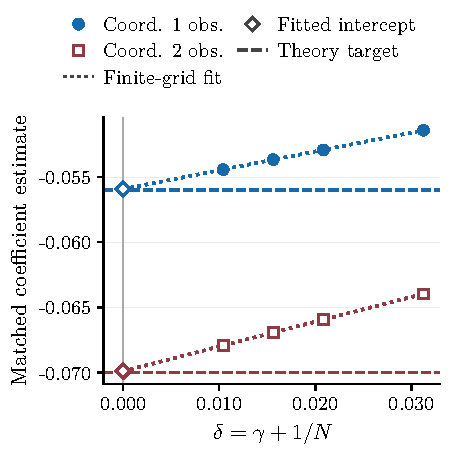
\includegraphics[width=\linewidth]{figures/redrawn/hist_H4_smallstep.pdf}
\caption{Smaller-step path}
\end{subfigure}\hfill
\begin{subfigure}[t]{0.49\textwidth}
\centering
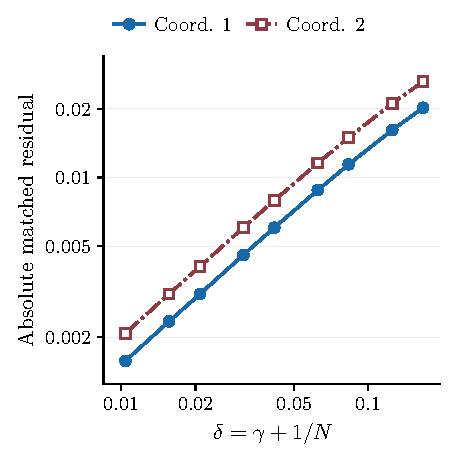
\includegraphics[width=\linewidth]{figures/redrawn/hist_H4_loglog_residual.pdf}
\caption{Absolute residuals}
\end{subfigure}
\caption{Matched $H=4$ finite-grid sensitivity.
(a) Smaller-step estimates (circles and squares), finite-grid linear fits
(dotted), and analytical targets (dashed). Open diamonds at $\delta=0$
mark the fitted intercepts.
(b) Absolute residuals versus $\delta=\gamma+1/N$ across all nine points
on logarithmic axes; lines connect the observed residuals.
The scaled residuals and log--log slopes are given in
Table~\ref{tab:E-h4diag}. Pointwise bars in (a) use simultaneous
Student-$t$ intervals; intercept bars use seed-block-bootstrap intervals.}
\label{fig:E-control-h4}
\label{fig:E-h4diag}
\end{figure}

\subsubsection{Fixed-step and five-dimensional results}
\label{app:num-supporting-results}

\paragraph{Design and rationale.}
These studies separately examine client count and dimension using the
objective family in Equation~\eqref{eq:num-objective}. The fixed-step
study uses the grid in Table~\ref{tab:num-controlled-settings}.
The five-dimensional instance has positive-definite $A,C$ with
$\|AC-CA\|_F=0.0876171216$.

\paragraph{Results and interpretation.}
Table~\ref{tab:E-plateau} adds the fixed-step intercept intervals and
offsets to Figure~\ref{fig:E-p2-plateau}. Table~\ref{tab:E-d5} supplies
all five coordinates for each local-step count. These details support
the client-count and multidimensional interpretations in
Sections~\ref{sec:num-supporting} and~\ref{sec:num-multidimensional}.

\begin{table}[tbp]
\centering\small
\caption{Sampling intervals and offsets for the fixed-step extrapolated
intercepts in Figure~\ref{fig:E-p2-plateau}.}
\label{tab:E-plateau}
\begin{tabular}{@{}clr@{}}
\toprule
$j$ & 95\% simultaneous CI & Intercept $-$ theory \\
\midrule
1 & $[-0.0489079,-0.0483504]$ & $-0.0006102$ \\
2 & $[-0.0607622,-0.0600656]$ & $-0.0003902$ \\
\bottomrule
\end{tabular}
\end{table}

\begin{table}[tbp]
\centering\small
\setlength{\tabcolsep}{4pt}
\caption{Five-dimensional \Scaf{} coefficient targets, fitted
intercepts, and nominal simultaneous 95\% bootstrap intervals.}
\label{tab:E-d5}
\begin{tabular}{@{}ccrrl@{}}
\toprule
$H$ & $j$ & $\widehat\beta_{0,j}$ & Theory & 95\% simultaneous CI \\
\midrule
2 & 1 & $-0.0140655061$ & $-0.0140249988$ & $[-0.0142709800,-0.0138295249]$ \\
2 & 2 & $-0.0457104417$ & $-0.0455796216$ & $[-0.0463785328,-0.0449434842]$ \\
2 & 3 & $ 0.0322203570$ & $ 0.0321284384$ & $[ 0.0316797243, 0.0326913914]$ \\
2 & 4 & $-0.0340954937$ & $-0.0339978616$ & $[-0.0345938212,-0.0335234201]$ \\
2 & 5 & $ 0.0160014114$ & $ 0.0159557997$ & $[ 0.0157329196, 0.0162353381]$ \\
\midrule
4 & 1 & $-0.0444005615$ & $-0.0444124962$ & $[-0.0446094313,-0.0441636371]$ \\
4 & 2 & $-0.1441927099$ & $-0.1443354682$ & $[-0.1448724780,-0.1434224100]$ \\
4 & 3 & $ 0.1016052163$ & $ 0.1017400551$ & $[ 0.1010621370, 0.1020846930]$ \\
4 & 4 & $-0.1075543334$ & $-0.1076598952$ & $[-0.1080613670,-0.1069797680]$ \\
4 & 5 & $ 0.0504598160$ & $ 0.0505266990$ & $[ 0.0501901098, 0.0506979332]$ \\
\bottomrule
\end{tabular}
\end{table}

\subsubsection{Leading-coefficient and restricted-grid sensitivity}
\label{app:supp-controlled}

\paragraph{Design and rationale.}
The independent fits estimate the common leading coefficient directly.
Restricted-grid comparisons omit the largest step size or, for the
matched control fits, the smallest client count. This assesses sensitivity
to points farther from the joint asymptotic limit.

\paragraph{Results and interpretation.}
Table~\ref{tab:supp-leading} gives the individual leading-intercept
estimates, complementing the matched results in
Table~\ref{tab:supp-control}. The $H=8$ offsets persist as a sensitivity
issue even when restricted fits move toward the targets. Primary estimates
remain the basis of the comparisons in Section~\ref{sec:num-supp-theory}.

\begin{table}[tbp]
\centering\small
\caption{Independent leading-coefficient fits with nominal 95\% intervals.
S: SCAFFOLD; F: FedAvg. The targets are
$B_{11,1}=-0.02445943$ and $B_{11,2}=-0.03057429$ for every $H$;
$H=1$ checks the boundary recursion.}
\label{tab:supp-leading}
\begin{tabular}{@{}ccrlrl@{}}\toprule
$H$ & Alg. & Estimate$_1$ & Interval$_1$ & Estimate$_2$ & Interval$_2$ \\ \midrule
1 & S & $-0.024531$ & $[-0.024960,-0.024102]$ & $-0.030664$ & $[-0.031200,-0.030127]$ \\
1 & F & $-0.024531$ & $[-0.024960,-0.024102]$ & $-0.030664$ & $[-0.031200,-0.030127]$ \\
2 & S & $-0.024432$ & $[-0.025068,-0.023795]$ & $-0.030554$ & $[-0.031349,-0.029758]$ \\
2 & F & $-0.024413$ & $[-0.025051,-0.023774]$ & $-0.030525$ & $[-0.031323,-0.029728]$ \\
4 & S & $-0.025169$ & $[-0.025953,-0.024385]$ & $-0.031537$ & $[-0.032517,-0.030557]$ \\
4 & F & $-0.024799$ & $[-0.025574,-0.024024]$ & $-0.031044$ & $[-0.032013,-0.030075]$ \\
8 & S & $-0.028252$ & $[-0.029046,-0.027459]$ & $-0.035610$ & $[-0.036602,-0.034618]$ \\
8 & F & $-0.025913$ & $[-0.026712,-0.025114]$ & $-0.032560$ & $[-0.033559,-0.031562]$ \\
\bottomrule\end{tabular}\end{table}

\subsubsection{Contraction and noise-law resolution}
\label{app:targeted-results}

\paragraph{Design and rationale.}
The supplementary comparisons assess how the matched result relates to
individual coefficients, the second coordinate, and restricted grids.
All use the model and resolution margins in
Appendix~\ref{app:targeted-model}. The signed-covariance contrast
subtracts the $\rho=-1/4$ symmetric condition from $\rho=1/4$.

\paragraph{Results and interpretation.}
Table~\ref{tab:mechanism-complement} supplements the matched
first-coordinate results in Table~\ref{tab:mechanism-controls}.
The paired signed-covariance estimates and simultaneous intervals are
\[
\begin{aligned}
 j=1:&\quad -0.04372973,\qquad [-0.04378778,-0.04367168],\\
 j=2:&\quad -0.00002676,\qquad [-0.00005541,0.00000188],
\end{aligned}
\]
against target $(-0.04375,0)^\top$. Individual first-coordinate null
and noise-law intervals are wider than their resolution bands, so the
precision gain is concentrated in the paired increment.

\begin{table}[!htbp]
\centering\small
\setlength{\tabcolsep}{3pt}
\caption{Additional contraction and noise-law results: individual coefficients
and contrasts, and the paired second coordinate. Estimates and interval
endpoints are multiplied by $10^3$.
S: \Scaf{}; F: \FedAvg{}; D: matched difference.
Targets follow Equation~\eqref{eq:targeted-coefficients}.
The law contrast is symmetric minus asymmetric at $\rho=1/4$;
the covariance contrast is $\rho=1/4$ minus $-1/4$ with symmetric noise.
Intervals use the primary family in Table~\ref{tab:mechanism-controls}.}
\label{tab:mechanism-complement}
\begin{tabular}{@{}lcrlrl@{}}
\toprule
Condition / contrast & Alg. & Estimate$_1$ & Interval$_1$ & Estimate$_2$ & Interval$_2$ \\
\midrule
$-1/4$, sym. & S & $56.0908$ & $[42.4573,\ 69.7243]$ & $2.6156$ & $[-4.5559,\ 9.7871]$ \\
$-1/4$, sym. & F & $34.2122$ & $[20.5757,\ 47.8487]$ & $2.6118$ & $[-4.5609,\ 9.7844]$ \\
\addlinespace
$0$, sym. & S & $4.6861$ & $[-18.0942,\ 27.4663]$ & $2.4973$ & $[-6.0117,\ 11.0064]$ \\
$0$, sym. & F & $4.7066$ & $[-18.0689,\ 27.4822]$ & $2.5118$ & $[-5.9994,\ 11.0230]$ \\
\addlinespace
$+1/4$, sym. & S & $-46.8325$ & $[-67.9207,\ -25.7443]$ & $2.2185$ & $[-4.0669,\ 8.5038]$ \\
$+1/4$, sym. & F & $-24.9813$ & $[-46.0714,\ -3.8913]$ & $2.2414$ & $[-4.0463,\ 8.5291]$ \\
\addlinespace
$+1/4$, asym. & S & $-58.1461$ & $[-81.4153,\ -34.8769]$ & $2.7156$ & $[-4.1149,\ 9.5460]$ \\
$+1/4$, asym. & F & $-36.2643$ & $[-59.5301,\ -12.9986]$ & $2.7160$ & $[-4.1137,\ 9.5457]$ \\
\addlinespace
Law contrast & S & $11.3136$ & $[-20.1352,\ 42.7624]$ & $-0.4971$ & $[-9.8863,\ 8.8921]$ \\
Law contrast & F & $11.2830$ & $[-20.1627,\ 42.7287]$ & $-0.4747$ & $[-9.8649,\ 8.9156]$ \\
\addlinespace
Covariance contrast & S & $-102.9233$ & $[-127.9666,\ -77.8799]$ & $-0.3971$ & $[-9.8315,\ 9.0372]$ \\
Covariance contrast & F & $-59.1935$ & $[-84.2420,\ -34.1451]$ & $-0.3704$ & $[-9.8073,\ 9.0665]$ \\
\addlinespace
\midrule
\multicolumn{6}{@{}l}{Additional paired second-coordinate results (zero target)} \\
$-1/4$, sym. & D & \multicolumn{2}{c}{---} & $0.0038$ & $[-0.0175,\ 0.0251]$ \\
$0$, sym. & D & \multicolumn{2}{c}{---} & $-0.0145$ & $[-0.0349,\ 0.0059]$ \\
$+1/4$, sym. & D & \multicolumn{2}{c}{---} & $-0.0229$ & $[-0.0423,\ -0.0035]$ \\
$+1/4$, asym. & D & \multicolumn{2}{c}{---} & $-0.0005$ & $[-0.0213,\ 0.0204]$ \\
Law contrast & D & \multicolumn{2}{c}{---} & $-0.0224$ & $[-0.0511,\ 0.0062]$ \\
\bottomrule
\end{tabular}
\end{table}

\paragraph{Restricted-grid sensitivity.}
Table~\ref{tab:num-restricted-mechanism} records the three restricted-grid
comparisons whose simultaneous intervals narrowly exclude their targets.
The two individual coefficient estimates lose sign resolution.
All three corresponding Bonferroni-$t$ intervals include the targets,
showing sensitivity to the interval construction as well as the grid.

\begin{table}[tbp]
\centering\small
\setlength{\tabcolsep}{4pt}
\caption{First-coordinate sensitivity after removing the largest step
in the contraction study. The first two rows use $\rho=1/4$ and symmetric
noise; the last row is the signed-covariance contrast.}
\label{tab:num-restricted-mechanism}
\begin{tabular}{@{}lrrl@{}}
\toprule
Quantity & Target & Estimate & Simultaneous interval \\
\midrule
\Scaf{} coefficient & $-0.059375$ & $-0.01675171$ & $[-0.05907084,0.02556741]$ \\
\FedAvg{} coefficient & $-0.0375$ & $0.00510137$ & $[-0.03721159,0.04741432]$ \\
\Scaf{} covariance contrast & $-0.11875$ & $-0.06840058$ & $[-0.11872928,-0.01807187]$ \\
\bottomrule
\end{tabular}
\end{table}

For the $\rho=1/4$ symmetric paired second coordinate, the primary
interval excludes zero but is contained in the resolution band. Its
Bonferroni-$t$ and restricted-grid intervals include zero. Reflection
symmetry of this objective and symmetric-noise recursion fixes the ideal
second-coordinate mean at zero from zero initial states. The small
empirical offset therefore probes finite-simulation and interval accuracy,
while the resolution-band comparison measures the size of that offset.

First/last-half balance comparisons give eight nominal 95\% exclusions
among 144 scalar diagnostics, all in individual algorithms; paired
intervals contain zero. Direct means have substantially larger sampling
variation than balance estimates. The diagnostics assess complementary
sources of uncertainty: window comparisons assess temporal variation,
finite-window identities assess arithmetic and alignment, and restricted
fits assess grid sensitivity. Stationary approximation remains unresolved.

\subsection{Estimator and structural consistency checks}
\label{app:num-consistency}

\subsubsection{Direct--balance estimator checks}
\label{app:direct-balance-diagnostic}

\paragraph{Design and rationale.}
The direct global mean provides a cross-check of the primary nonlinear
balance observable. The unnormalized diagnostic is
\[
 |\widehat b_{{\rm direct},j}-\widehat b_{{\rm bal},j}|
 \le3\operatorname{SE}_{\rm comb},\qquad
 \operatorname{SE}_{\rm comb}
 =\sqrt{\operatorname{SE}_{{\rm direct},j}^2+
         \operatorname{SE}_{{\rm bal},j}^2}.
\]
Using the unnormalized means keeps the comparison on the parameter scale;
second-order normalization multiplies estimation errors by $\gamma^{-2}$.

\paragraph{Results and interpretation.}
The primary two-dimensional \FedAvg{} study satisfies the diagnostic in
156 of 160 chain-coordinate checks. Table~\ref{tab:E-direct-balance}
gives the four exceptions; their discrepancy-to-threshold ratios are
$1.137$, $1.164$, $1.108$, and $1.060$. All checks satisfy the criterion
in the two-dimensional \Scaf{} studies, fixed-step study,
five-dimensional \Scaf{} study, and smaller-step \FedAvg{} study.
These counts concern the individual algorithms. In the independent
controlled study, four of 68 algorithm--configuration raw-versus-balance
intervals exclude zero. The primary estimates throughout use the
balance observable.

\begin{table}[tbp]
\centering\small
\setlength{\tabcolsep}{3pt}
\caption{The four direct--balance discrepancies in the primary
\FedAvg{} study. The diagnostic uses the unnormalized difference
$|\Delta\widehat b|$; the normalized statistics are also shown.}
\label{tab:E-direct-balance}
\begin{tabular}{@{}cccrrrr@{}}
\toprule
$H$ & $N$ & $j$ & $\widehat C_{\rm bal}$ & $\widehat C_{\rm dir}$ &
$|\Delta\widehat b|$ & $3\operatorname{SE}_{\rm comb}$ \\
\midrule
2 & 16 & 2 &
$-0.0408082$ & $ 0.924598$ & $0.00377112$ & $0.00331567$ \\
2 & 48 & 1 &
$-0.0323449$ & $ 3.070686$ & $0.00134680$ & $0.00115744$ \\
4 & 16 & 2 &
$-0.1080240$ & $ 0.841309$ & $0.00370833$ & $0.00334677$ \\
4 & 48 & 1 &
$-0.0933450$ & $ 2.615233$ & $0.00117560$ & $0.00110953$ \\
\bottomrule
\end{tabular}
\end{table}

Reanalysis of the existing $H=4$ Cartesian-grid runs gives paired
raw-minus-balance fitted-intercept differences of
$-2.39\times10^{-7}$ and $-2.92\times10^{-7}$. The paired intercepts
therefore change little under estimator substitution. Finite-window
identities agree where endpoints are available. Missing endpoints and
individual noise sums limit this check to those windows; the joint-grid
$H=4$ discrepancy remains as reported in
Appendix~\ref{app:num-h4-diagnostics}.

\subsubsection{Orthogonal coordinate equivariance}
\label{app:equivariance-check}
\label{app:equivariance}

\paragraph{Design and rationale.}
A coordinate change should transform the complete recursion and its
coefficient vectors consistently. For $y=Qx$ with $QQ^\top=I$, set
$A_y=QAQ^\top$, $C_y=QCQ^\top$, and $S_{C,y}=QS_CQ^\top$.
The Lyapunov equation becomes $A_yS_{C,y}+S_{C,y}A_y=C_y$, and
\begin{equation}
\label{eq:D-tensor-equiv}
 T_y[QMQ^\top]=QT[M]
 \quad\text{for every symmetric }M.
\end{equation}
The coefficient formulas then give
\begin{equation}
\label{eq:D-coefficient-equivariance}
 B_{11,y}=QB_{11},\qquad
 B_{20,y}^{a}(H)=QB_{20}^{a}(H),\quad
 a\in\{\Scaf,\FedAvg,\mathrm{ctrl}\}.
\end{equation}
The simulation applies the same transformation to every noise draw.
Table~\ref{tab:num-structural-settings} lists the rotation and affine
comparison settings.

\begin{table}[tbp]
\centering\small
\setlength{\tabcolsep}{4pt}
\caption{Structural consistency checks. Corresponding initial states and
noise realizations are used within each comparison.}
\label{tab:num-structural-settings}
\begin{tabularx}{\linewidth}{@{}>{\raggedright\arraybackslash}p{0.22\linewidth}>{\raggedright\arraybackslash}X@{}}
\toprule
Check & Configuration \\
\midrule
Orthogonal rotation &
$Q=\left(\begin{smallmatrix}0.8660254037844386&-0.5\\0.5&0.8660254037844386\end{smallmatrix}\right)$ ($30^\circ$);
$H\in\{2,4\}$; $(N,\gamma)\in\{(16,1/16),(64,1/64)\}$;
4 paired runs per configuration, 16 paths in total \\
Affine translation &
$N\in\{8,32\}$; $H\in\{2,4,8\}$;
$a_c=\pm\rho u$, $\rho\in\{0,0.25,0.5,1\}$;
$\gamma=1/128$; 24 configurations of 2,000 rounds \\
\bottomrule
\end{tabularx}
\end{table}

\paragraph{Results and interpretation.}
The full-path residuals satisfy
\[
 \max_t\|x_t^{(y)}-Qx_t^{(x)}\|_\infty\le1.1491\times10^{-14},\qquad
 \max_{t,c}\|\xi_{t,c}^{(y)}-Q\xi_{t,c}^{(x)}\|_\infty\le1.5765\times10^{-14},
\]
with $\max_{t,h}\|\bar q_{t,h}^{(y)}-Q\bar q_{t,h}^{(x)}\|_\infty
\le5.4210\times10^{-17}$ and coefficient residuals below
$6\times10^{-16}$. All are within the $10^{-10}$ tolerance,
confirming coordinate consistency of the \Scaf{} implementation.

\subsubsection{Affine translation and update identities}
\label{app:num-affine-checks}

\paragraph{Design and rationale.}
The affine comparisons use balanced gradient offsets and the translated
initial controls prescribed by Proposition~\ref{prop:affine-shift}.
With common noise, the transformed states should agree at every round.
Zero initialization in both untransformed systems gives different
transients because the initial states are no longer translated counterparts.
Long-run $H=1$ checks separately assess arithmetic accumulation.

\paragraph{Results and interpretation.}
The affine residual reported in Section~\ref{sec:num-affine} reproduces
the exact translation to numerical precision. Short-run update-identity
checks also pass. Over longer runs, 48 of 132 $H=1$ arithmetic checks
exceed $10^{-10}$, with maximum vector discrepancy about
$7.54\times10^{-10}$. The shared-objective subset has 24 exceedances
among 60 checks and maximum coordinate discrepancy $4.33\times10^{-10}$.
Two additional paths using a stable endpoint-increment calculation reduce
vector discrepancies to about $10^{-12}$. This improvement is documented
for those two paths; the original full-grid outputs remain the reported
results.

\subsection{Real-data analyses and diagnostics}
\label{app:num-real-analyses}

\subsubsection{Objectives, partitions, and allocation estimands}
\label{app:supp-real}

\paragraph{Design and rationale.}
The shared-objective comparison isolates allocation effects, while disjoint
partitions introduce heterogeneous local objectives. We use the a9a
training and test sets from the LIBSVM collection.\footnote{\url{https://www.csie.ntu.edu.tw/~cjlin/libsvmtools/datasets/binary.html}}
Table~\ref{tab:num-real-settings} collects preprocessing, training, and
averaging settings. Each client minimizes
\begin{equation}
\label{eq:real-objective}
f_c(x)=\frac1{|D_c|}\sum_{i\in D_c}\{\log(1+e^{z_i^\top x})-y_i z_i^\top x\}+\frac{\lambda}{2}\|x\|^2.
\end{equation}
Equal client weights preserve the global empirical objective. The
shared-objective reference aggregate covariance has trace $0.001060$
after rounding; disjoint partitions can change reference covariances and
local objectives, including under IID assignment.

\begin{table}[tbp]
\centering\small
\setlength{\tabcolsep}{4pt}
\caption{Real-data settings. All training configurations use twelve
independent \Scaf{}--\FedAvg{} pairs. Windows within a run share its
trajectory. The two longer-run pilots are analyzed separately.}
\label{tab:num-real-settings}
\begin{tabularx}{\linewidth}{@{}>{\raggedright\arraybackslash}p{0.30\linewidth}>{\raggedright\arraybackslash}X@{}}
\toprule
Component & Specification \\
\midrule
Training data &
32,512 of 32,561 rows selected by a fixed random permutation to allow equal disjoint partitions \\
Features and penalty &
Each 123-feature row divided by $\max\{1,\|z_i\|\}$, then augmented with an intercept;
$y_i\in\{0,1\}$; all 124 parameters regularized with $\lambda=0.01$ \\
Client objectives &
Shared: all clients use the same data; disjoint IID: random partition;
label skew: two label-sorted shards per client.
Disjoint regimes use one primary and two alternative partitions \\
Minibatches and base step &
Sampling with replacement; $L_{\rm sample}=0.51$;
$\gamma_b=0.1/L_{\rm sample}=0.1960784314$ \\
Fixed-budget allocations &
$Nm=256$; $(N,m)\in\{(8,32),(32,8),(128,2)\}$;
$H=4$, $\gamma=\gamma_b$ \\
Additional shared-objective runs &
Three step-size/local-step variants (Table~\ref{tab:supp-policy}) and three $H=1$ checks;
nine shared-objective configurations in total \\
Averaging windows &
$K\in\{1,2,4,8,16,32,64\}$ final batches per run;
primary configuration $H=4,N=128,m=2,\gamma_b$ \\
Primary averaging horizon &
1,280 rounds per batch; 6,400 burn-in rounds;
longest window 81,920 rounds, ending at round 88,320;
90,439,680 example-gradient evaluations per algorithm \\
Longer-run pilots &
Two runs; 25,600 burn-in rounds and 128 batches of 1,280 rounds;
189,440 rounds per run \\
\bottomrule
\end{tabularx}
\end{table}

The reference Newton solve has gradient norm $1.253\times10^{-16}$ and
strong-convexity parameter-error bound $1.253\times10^{-14}$; a separately
initialized solver differs by $8.43\times10^{-15}$. These floating-point
residuals quantify numerical accuracy of the reference used to evaluate
$A_{\rm ref}$, $T_{\rm ref}$, and $\Sigma_{\rm ref}$.
The projection direction in Equation~\eqref{eq:real-projection} is fixed
before training.

Squared mean displacement is estimated by $\widehat U_K$ in
Equation~\eqref{eq:e4-estimators} at the complete tail. Raw-checkpoint
MSE comes from separately accumulated squared errors; its variance estimate
subtracts the corresponding cross-run squared-mean estimate. Negative
sampling-corrected values are retained. The nominal jackknife-$t$ intervals
and adjusted contrast families are described in Table~\ref{tab:num-inference}.

\paragraph{Results and interpretation.}
Table~\ref{tab:supp-real-full} adds raw error and held-out loss results
to the main allocation study, and supplies the disjoint-partition results.
In the label-skew case at $N=32,H=4$, deterministic \FedAvg{} converges
to a point about $0.08365$ from $x_{\rm ref}$. The algorithm difference
therefore includes a substantial drift-correction effect in addition to
stochastic mean displacement.

The pointwise projection half-width target $10^{-4}$ is unmet in 32 of
35 real-data configurations, including the main shared-objective
allocations. The separately estimated allocation contrasts nevertheless
resolve their signed differences. Precision of an individual mean and
precision of a paired contrast are distinct features of the experiment.

\begin{table}[tbp]
\centering\small
\caption{Additional finite-tail allocation results at $H=4$, $\gamma_b$,
and $Nm=256$. The upper panel supplements Figure~\ref{fig:real-allocation}
with error and loss measurements; the lower panel reports disjoint
partitions. Projection intervals are nominal 95\% intervals.
Raw-checkpoint MSE is multiplied by $10^3$; held-out loss is averaged
over the per-run tail-average models. S: SCAFFOLD; F: FedAvg.}
\label{tab:supp-real-full}
\begin{tabular}{@{}crrrr@{}}
\toprule
\multicolumn{5}{c}{Shared objective: additional error and loss measurements} \\
$N$ & MSE (S) & MSE (F) & Test loss (S) & Test loss (F) \\
\midrule
8 & $2.3511$ & $2.3509$ & $0.424981$ & $0.424983$ \\
32 & $2.3629$ & $2.3618$ & $0.424961$ & $0.424970$ \\
128 & $2.3745$ & $2.3655$ & $0.424889$ & $0.424922$ \\
\bottomrule
\end{tabular}

\medskip
\begin{tabular}{@{}ccrlrr@{}}
\toprule
$N$ & Alg. & Projection & Nominal interval & MSE & Test loss \\
\midrule
\multicolumn{6}{l}{\emph{Disjoint IID partition}} \\
8 & S & $0.000341$ & $[0.000213,0.000468]$ & $2.3458$ & $0.424978$ \\
8 & F & $0.000268$ & $[0.000140,0.000396]$ & $2.3454$ & $0.424981$ \\
32 & S & $0.000880$ & $[0.000638,0.001123]$ & $2.3661$ & $0.424963$ \\
32 & F & $0.000472$ & $[0.000230,0.000715]$ & $2.3643$ & $0.424977$ \\
128 & S & $0.003553$ & $[0.003393,0.003714]$ & $2.3642$ & $0.424884$ \\
128 & F & $0.001994$ & $[0.001830,0.002158]$ & $2.3507$ & $0.424936$ \\
\midrule
\multicolumn{6}{l}{\emph{Disjoint label-skew partition}} \\
8 & S & $0.000243$ & $[0.000050,0.000436]$ & $2.2526$ & $0.424984$ \\
8 & F & $-0.039298$ & $[-0.039491,-0.039104]$ & $5.6791$ & $0.426589$ \\
32 & S & $0.000352$ & $[0.000143,0.000561]$ & $2.2180$ & $0.424981$ \\
32 & F & $-0.055891$ & $[-0.056096,-0.055686]$ & $9.0666$ & $0.427274$ \\
128 & S & $0.001256$ & $[0.001096,0.001416]$ & $2.1956$ & $0.424956$ \\
128 & F & $-0.062027$ & $[-0.062182,-0.061872]$ & $10.7951$ & $0.427548$ \\
\bottomrule
\end{tabular}
\end{table}

\subsubsection{Run-length sensitivity}
\label{app:supp-audit}

\paragraph{Design and rationale.}
First/last-half comparisons assess variation within the recorded tails.
They use the same 64-batch trajectories and the $2\times69$ adjustment
across controlled and real-data projected contrasts. In the shared-objective
real-data study, the primary observable is the direct mean itself.

\paragraph{Results and interpretation.}
The adjusted first/last-half contrast intervals contain zero. The endpoint
allocation contrasts in the first and last halves are $0.003098$ and
$0.003129$ for \Scaf{}, and $0.002053$ and $0.002092$ for \FedAvg{}.
The similar values support stability of the allocation comparison within
the sampled tails. The stronger temporal-equivalence criterion is assessed
separately below.

\subsubsection{Finite-tail model averaging}
\label{app:e4-averaging}

\paragraph{Design and rationale.}
To quantify the components in Equation~\eqref{eq:e4-finite-window-mse},
set $e_{r,K}^{\mathcal A}=Y_{r,K}^{\mathcal A}-x_{\rm ref}$ and
$\bar e_K=R^{-1}\sum_r e_{r,K}$ with $R=12$.
Suppressing the algorithm superscript,
\begin{equation}
\label{eq:e4-estimators}
\widehat U_K=\frac{\sum_{r\ne s}e_{r,K}^{\top}e_{s,K}}{R(R-1)},\qquad
\widehat V_K=\frac{\sum_r\|e_{r,K}-\bar e_K\|^2}{R-1},\qquad
\widehat M_K=\frac1R\sum_r\|e_{r,K}\|^2=\widehat U_K+\widehat V_K.
\end{equation}
Cross-products between independent runs estimate the squared mean
displacement, while between-run deviations estimate the variance of the
time-averaged outputs. The estimators retain negative values of
$\widehat U_K$. Training and test losses are evaluated on each run's own
$Y_{r,K}$ and then averaged across runs.

The primary, secondary, and additional configurations use the schedules
in Table~\ref{tab:num-real-settings}. The $N=8,32$ allocations are
secondary; six further configurations examine step size, local steps,
and $H=1$. Bootstrap resampling uses one common run-index vector across
algorithms, configurations, and overlapping windows. Separate uncertainty
families are listed in Table~\ref{tab:num-inference}; all condition on
the fixed dataset and recorded finite-tail protocol.

\paragraph{Results and interpretation.}
Table~\ref{tab:e4-primary} gives absolute errors and losses complementing
the main-text error shares. For $b_S=b_F+\delta$, the difference in squared
means obeys $\|b_S\|^2-\|b_F\|^2=2b_F^\top\delta+\|\delta\|^2$.
The sampling-corrected decomposition is
$\Delta\widehat U=2(2.57965\times10^{-6})+1.21856\times10^{-6}$,
showing the contribution of both the cross term and the squared algorithmic
displacement. The total-MSE contrast corresponds to a $58.7\%$ relative
difference. For scale, $f(x_{\rm ref})=0.4758413$ and the held-out contrast
has magnitude about $0.00769\%$ of reference test loss.

\begin{table}[t]
\centering\small
\caption{Additional longest-window model-averaging statistics at $K=64$,
with approximate simultaneous 95\% primary-family intervals.
Parameter errors and training gaps are multiplied by $10^6$;
test loss is unscaled. The component shares and total-MSE contrast
are reported in Section~\ref{sec:num-averaging}.}
\label{tab:e4-primary}
\begin{tabular}{@{}lrr@{}}
\toprule
Quantity & SCAFFOLD & FedAvg \\
\midrule
$\widehat M_K$ & $17.267\ [15.383, 19.151]$ & $10.878\ [9.459, 12.297]$ \\
Train objective gap & $0.725\ [0.630, 0.819]$ & $0.361\ [0.295, 0.426]$ \\
Held-out log loss & $0.424889\ [0.424879, 0.424899]$ & $0.424922\ [0.424912, 0.424932]$ \\
\midrule
Paired difference & \multicolumn{2}{c}{Estimate [simultaneous interval]} \\
$\Delta\widehat U_K$ & \multicolumn{2}{c}{$6.378\ [5.848, 6.908]$} \\
$\Delta\widehat V_K$ & \multicolumn{2}{c}{$0.011\ [-0.036, 0.058]$} \\
\midrule
\multicolumn{3}{l}{Additional intervals for the loss contrasts reported in the main text:} \\
$\Delta$ train gap & \multicolumn{2}{c}{$[0.336, 0.393]$} \\
$\Delta$ held-out log loss & \multicolumn{2}{c}{$[-0.00003308, -0.00003231]$} \\
\bottomrule
\end{tabular}
\end{table}

At $N=32$ and $8$, the longest-window \Scaf{}/\FedAvg{} mean-displacement
shares are $14.97\%/7.77\%$ and $1.61\%/0.97\%$, respectively.
Their squared-mean intervals give weaker evidence against zero than the
primary allocation. Together with the main result, these comparisons show
that the error share depends on allocation as well as averaging length.

\paragraph{Temporal diagnostics.}
The predeclared equivalence test requires both a $10^{-3}$ vector-norm
margin and a $10^{-4}$ projected-drift margin. None of 144 checks meets
both requirements. In the primary \Scaf{} comparison, the first/last
32-batch drift norm is $0.0013633$, with upper bound $0.0054372$ and
projected interval $[-0.0005438,0.0007484]$. The longest window inherits
the 32-batch check because a separate equal-length 64-batch anchor is
unavailable. Thus temporal equivalence remains unresolved.

For \Scaf{}, $\widehat U_K\geq\widehat V_K$ at $K=32,64$, with a
positive lower bound for $U-V$ under both interval procedures only at
$K=64$. The prespecified crossover requirement---two consecutive supported
windows together with temporal equivalence---is unmet. \FedAvg{} has
no point-estimate crossover on this grid. The protocol's $10\%$
parameter-MSE-share threshold is a researcher-chosen reference.
The two longer-run pilots in Table~\ref{tab:num-real-settings} leave
these temporal questions unresolved. The established result is the
finite-tail error decomposition reported in Section~\ref{sec:num-averaging}.

\subsubsection{Post-hoc directional comparison}
\label{app:e5-bridge}

\paragraph{Design and rationale.}
To contextualize the alignment in Table~\ref{tab:e5-bridge}, we compare
the analytical direction with the fixed reference-parameter direction
and the unpreconditioned vector $-T_{\rm ref}[\Sigma_{\rm ref}]$.
Window, step-size, and local-step comparisons assess how alignment and
amplitude change within the existing runs. The zero-vector proxy supplies
an amplitude baseline. Sampling procedures are listed in
Table~\ref{tab:num-inference}; scalar and vector families each have their
own 95\% calibration.

\paragraph{Results and interpretation.}
At $K=64$, reference-parameter cosines are $0.8953$--$0.9087$ and
unpreconditioned-direction cosines are $0.6590$--$0.6929$.
Both are lower than the analytical proxy values in the main table; the
zero-vector proxy also has larger residuals in all six configurations.
These comparisons make the geometric agreement specific to the
Hessian-preconditioned curvature--noise direction among the tested references.

For the fixed-$H,N,m$ sequence, adjacent log slopes of the observed
projection are $1.8553$ and $1.8907$. Across shorter averaging windows,
the cosine falls as low as $0.872197$. These results describe finite-grid
and window sensitivity. Allocation comparisons change $N$ and $m$
together, preserving total sampling budget while changing local covariance.

For the $H=4/H=2$ ratio in Section~\ref{sec:num-directional}, the
exploratory simultaneous interval is $[2.7415,3.1125]$, the jackknife
interval is $[2.7101,3.1439]$, and the projection-band transform is
$[2.6928,3.1919]$. All exclude $3.5$ and include the ordinary local-update
ratio $3$. The results resolve a departure from the plug-in local-step
scaling; attribution of that departure remains open. The $H=1$ residuals
are approximately $10^{-11}$--$10^{-10}$, consistent with the expected
zero-proxy numerical identity.

The 54 early/late paired contrasts assess temporal variation of the
algorithm difference. The model-averaging diagnostics in
Appendix~\ref{app:e4-averaging} assess each algorithm separately, so
the two comparisons address different temporal quantities. The proxy
agreement remains a descriptive geometric result for the recorded
finite-tail means.
